\documentclass[11pt]{article}
\usepackage[title]{appendix}
\usepackage[utf8]{inputenc}
\usepackage[english]{babel}
\usepackage{graphicx}
\usepackage{float}
\usepackage{amssymb,amsmath}
\usepackage{mathtools}
\usepackage{xcolor}
\usepackage{xspace}
%\usepackage[]{algorithm2e}
\usepackage{algorithm}
%\usepackage{algorithmic}
%\usepackage{algpseudocode}
\usepackage[noend]{algpseudocode}
\usepackage{caption}
\usepackage{marginnote}
%
\usepackage{amssymb,amsmath}%,amsthm}
% \usepackage{subfigure}
% \usepackage{amsmath}
\usepackage{amsfonts}
\usepackage{amsthm}
\usepackage{upgreek}

% \newtheorem{assumption}{Assumption}
% \theoremstyle{definition}
% \newtheorem{definition}{Definition}[section]
% \newtheorem{definition}{Definition}
% \newtheorem{lemma}{Lemma}
% \newtheorem{theorem}{Theorem}
% \newtheorem{proposition}{Proposition}
% % \newtheorem{proof}{Proof}
% \newtheorem{remark}{Remark}

% New stuff added by Sayan
%% Some standard libraries
\usepackage{paralist}
\usepackage{xspace}

\DeclareMathOperator*{\argmax}{arg\,max}
\DeclareMathOperator*{\argmin}{arg\,min}
\theoremstyle{definition}
\newtheorem{thm}{Theorem}
\newtheorem{prop}{Proposition}

\newtheorem{definition}{Definition}
\newtheorem{lemma}{Lemma}
\newtheorem{theorem}{Theorem}
\newtheorem{proposition}{Proposition}
% \newtheorem{proof}{Proof}
\newtheorem{remark}{Remark}

\newcommand{\sayan}[1]{\textcolor{blue}{#1}}
\newcommand{\negin}[1]{\textcolor{magenta}{#1}}
\newcommand{\geir}[1]{\textcolor{red}{#1}}
\newcommand{\dawei}[1]{\textcolor{green}{#1}}

%% Defining some Macros to be used throughout the paper


\newcommand{\num}[1]{\relax\ifmmode \mathbb #1\else $\mathbb #1$\fi}
\newcommand{\nnnum}[1]{\relax\ifmmode
  {\mathbb #1}_{\geq 0} \else ${\mathbb #1}_{\geq 0}$
  \fi}
\newcommand{\npnum}[1]{\relax\ifmmode
  {\mathbb #1}_{\leq 0} \else ${\mathbb #1}_{\leq 0}$
  \fi}
\newcommand{\pnum}[1]{\relax\ifmmode
  {\mathbb #1}_{> 0} \else ${\mathbb #1}_{> 0}$
  \fi}
\newcommand{\nnum}[1]{\relax\ifmmode
  {\mathbb #1}_{< 0} \else ${\mathbb #1}_{< 0}$
  \fi}
\newcommand{\plnum}[1]{\relax\ifmmode
  {\mathbb #1}_{+} \else ${\mathbb #1}_{+}$
  \fi}
\newcommand{\nenum}[1]{\relax\ifmmode
  {\mathbb #1}_{-} \else ${\mathbb #1}_{-}$
  \fi}

\newcommand{\bools}{{\num B}}                    %reals
\newcommand{\reals}{{\num R}}                    %reals
\newcommand{\nnreals}{{\nnnum R}}                    %nonnegative reals
\newcommand{\realsinfty}{{\num R} \cup \{\infty, -\infty\}}                    %nonnegative reals
\newcommand{\plreals}{{\plnum R}}                    %positive reals
\newcommand{\naturals}{{\num N}}                      %natural numbers
\newcommand{\integers}{{\num Z}}                      %integers
\newcommand{\nnintegers}{{\nnnum Z}}
\newcommand{\rationals}{{\num Q}}                      %rationals
\newcommand{\nnrationals}{{\nnnum Q}}                   % nonnegative rationals
\newcommand{\Time}{{\num T}}


\newcommand{\M}{\mathcal{M}}
\newcommand{\X}{\mathcal{X}}
\newcommand{\B}{\mathcal{B}}
\newcommand{\pack}{\mathcal{N}_{\mathit{pack}}}
\newcommand{\phit}[3]{{p_{#1,#2}{(#3)}}}

\newcommand{\observ}{y}
\newcommand{\Observ}{Y}
\newcommand{\Prob}{{\num P}}
\newcommand{\Trans}[3]{{#1}_{{#2,#3}}}
\newcommand{\Unsafe}{\mathcal{U}}
\newcommand{\uthresh}{\eta}
\newcommand{\supp}[1]{{\rm{supp}\mathit{(#1)}}}
\newcommand{\modelname}{NiMC\xspace}
\newcommand{\execs}[1]{{{\rm{Execs}}_{#1}}}
\newcommand{\partition}[2]{{\mathcal{P}_{#1,#2}}}
\newcommand{\counter}[2]{{\mathit{count}_{#1,#2}}}

\newcommand{\Scar}{{$\mathsf{Singlecar}$\xspace}}
\newcommand{\SlplatoonTwo}{{$\mathsf{SLplatoon2}$\xspace}}
\newcommand{\SlplatoonThree}{{$\mathsf{SLplatoon3}$\xspace}}
\newcommand{\Mlplatoon}{{$\mathsf{MLplatoon}$\xspace}}

\newcommand{\toolname}{{{\sf HooVer}\xspace}}


%% transition system quick description
\usepackage{listings}

\usepackage{stmaryrd}
\usepackage{multirow}
\usepackage{array}
\usepackage{upgreek}

\newcommand{\two}[4]{
  \parbox{.95\columnwidth}{\vspace{1pt} \vfill
    \parbox[t]{#1\columnwidth}{#3}%
    \parbox[t]{#2\columnwidth}{#4}%
  }}

\lstdefinelanguage{pseudocode}{
	basicstyle=\scriptsize,
	keywordstyle=\bf \scriptsize,
	identifierstyle=\it \scriptsize,
%	emphstyle=\tt \figuresize,
	mathescape=true,
	tabsize=20,
	xleftmargin=4.0ex,
	sensitive=false,
	columns=fullflexible,
	keepspaces=false,
	%flexiblecolumns=true,
	%  basewidth=0.5em,
	basewidth=0.05em,
	moredelim=[il][\rm]{//},
	moredelim=[is][\sf \figuresize]{!}{!},
	moredelim=[is][\bf \figuresize]{*}{*},
	keywords={automaton, algorithm, and,
		break,
		choose,const,continue, components,
		discrete, do,
		eff, external,else, elseif, evolve, end, each, exit,
		fi,for, forward, from, find,
		hidden,
		in,input,internal,if,invariant, initially, imports,
		let,
		mode,
		or, output, operators, od, of,
		pre,
		return,
		such,satisfies, stop, signature, simulation, sample,
		trajectories,trajdef, transitions, that,then, type, types, to, tasks,
		variables, vocabulary,
		when,where, with,while},
	emph={set, seq, tuple, map, array, enumeration},
	literate=
	{(}{{$($}}1
	{)}{{$)$}}1
	% LaTeX math symbols
	{\\in}{{$\in\ $}}1
	{\\preceq}{{$\preceq\ $}}1
	{\\subset}{{$\subset\ $}}1
	{\\subseteq}{{$\subseteq\ $}}1
	{\\supset}{{$\supset\ $}}1
	{\\supseteq}{{$\supseteq\ $}}1
	{\\forall}{{$\forall$}}1
	{\\le}{{$\le\ $}}1
	{\\ge}{{$\ge\ $}}1
	{\\gets}{{$\gets\ $}}1
	{\\cup}{{$\cup\ $}}1
	{\\cap}{{$\cap\ $}}1
	{\\langle}{{$\langle$}}1
	{\\rangle}{{$\rangle$}}1
	{\\exists}{{$\exists\ $}}1
	{\\bot}{{$\bot$}}1
	{\\rip}{{$\rip$}}1
	{\\emptyset}{{$\emptyset$}}1
	{\\notin}{{$\notin\ $}}1
	{\\not\\exists}{{$\not\exists\ $}}1
	{\\ne}{{$\ne\ $}}1
	{\\to}{{$\to\ $}}1
	{\\implies}{{$\implies\ $}}1
	% LSL symbols (one-character)
	{<}{{$<\ $}}1
	{>}{{$>\ $}}1
	{=}{{$=\ $}}1
	{~}{{$\neg\ $}}1
	{|}{{$\mid$}}1
	{'}{{$^\prime$}}1
	% LSL symbols (two characters)
	{\\A}{{$\forall\ $}}1
	{\\E}{{$\exists\ $}}1
	{\\/}{{$\vee\,$}}1
	{\\vee}{{$\vee\,$}}1
	{/\\}{{$\wedge\,$}}1
	{\\wedge}{{$\wedge\,$}}1
	{=>}{{$\Rightarrow\ $}}1
	{->}{{$\rightarrow\ $}}1
	{<=}{{$\Leftarrow\ $}}1
	{<-}{{$\leftarrow\ $}}1
	%        {<=}{{$\leq$}}1
	%        {>=}{{$\geq$}}1
	{~=}{{$\neq\ $}}1
	{\\U}{{$\cup\ $}}1
	{\\I}{{$\cap\ $}}1
	{|-}{{$\vdash\ $}}1
	{-|}{{$\dashv\ $}}1
	{<<}{{$\ll\ $}}2
	{>>}{{$\gg\ $}}2
	{||}{{$\|$}}1
	%%       {\[\]}{{\[\,\]}}2 {\{\}}{{\{\,\}}}2
	%%        {[}{{$\langle$}}1
	%%        {]}{{$\rangle$}}1
	{[}{{$[$}}1
	{]}{{$\,]$}}1
	{[[}{{$\langle$}}1
	{]]]}{{$]\rangle$}}1
	{]]}{{$\rangle$}}1
	{<=>}{{$\Leftrightarrow\ $}}2
	{<->}{{$\leftrightarrow\ $}}2
	{(+)}{{$\oplus\ $}}1
	{(-)}{{$\ominus\ $}}1
	{_i}{{$_{i}$}}1
	{_j}{{$_{j}$}}1
	{_{i,j}}{{$_{i,j}$}}3
	{_{j,i}}{{$_{j,i}$}}3
	{_0}{{$_0$}}1
	{_1}{{$_1$}}1
	{_2}{{$_2$}}1
	{_n}{{$_n$}}1
	{_p}{{$_p$}}1
	{_k}{{$_n$}}1
	{-}{{$\ms{-}$}}1
	{@}{{}}0
	{\\delta}{{$\delta$}}1
	{\\R}{{$\R$}}1
	{\\Rplus}{{$\Rplus$}}1
	{\\N}{{$\N$}}1
	{\\times}{{$\times\ $}}1
	{\\tau}{{$\tau$}}1
	{\\alpha}{{$\alpha$}}1
	{\\beta}{{$\beta$}}1
	{\\gamma}{{$\gamma$}}1
	{\\ell}{{$\ell\ $}}1
%	{--}{{$-\ $}}1
	{\\TT}{{\hspace{1.5em}}}3
}

\lstdefinelanguage{pseudocodeNums}[]{pseudocode}
{
	numbers=left,
	numberstyle=\tiny,
	stepnumber=2,
	numbersep=4pt
	%  firstnumber=1
}

%
% \usepackage{caption,subcaption}
% Sayan: had to remove subcaption because my latex compiler was complaining.
%\usepackage[dvipsnames]{xcolor}
\usepackage{fullpage}
\usepackage{hyperref}
\hypersetup{
	pdftitle={Optimistic Optimization for Statistical Model Checking with Regret Bounds},
	pdfauthor={Dawei Sun},
	colorlinks=true,
	citecolor={blue},
	linkcolor = {blue},
	pagecolor={blue},
	backref={true},
	bookmarks=true,
	bookmarksopen=false,
	bookmarksnumbered=true
}

%\newtheorem{problem}{Problem Statement}

%% End of stuff added by Sayan
%\baselineskip=10pt
\begin{document}

%\usepackage[a4paper, total={6in, 9in}]{geometry}
\title{Optimistic Optimization for Statistical Model Checking with Regret Bounds\\ ECE 584 Project Report}
\author{Negin Musavi$^1$, Dawei Sun$^1$, Sayan Mitra$^1$, Geir Dullerud$^1$, and Sanjay Shakkottai$^2$
\\
{\{nmusavi2,daweis2,mitras,dullerud\}@illinois.edu} \\ ${}^1$University of Illinois at Urbana Champaign \\
sanjay.shakkottai@utexas.edu
\\ ${}^2$University of Texas  at Austin}

%\titlerunning{Optimistic Optimization for Model Checking with Regrets}
%\authorrunning{Musavi, Sun, Mitra, Dullerud, and Shakkottai}

\maketitle

% Separating files for sections

%\input{abstract}
\begin{abstract}
We explore application of multi-armed bandit algorithms to  statistical model checking (SMC) of Markov chains initialized to a set of states.
%
We observe that model checking problems requiring  maximization of probabilities of sets of execution over all choices of the initial states, can be formulated as a multi-armed bandit problem, for appropriate costs and rewards. Therefore, the problem can be solved using   multi-fidelity hierarchical optimistic optimization (MFHOO).
%
%This class of models and requirements capture  practical problems in online monitoring where initialization has to consider  worst case errors from sensing and perception modules.
%
Bandit algorithms, and MFHOO in particular, give  (regret) bounds on the sample efficiency  which rely on the  smoothness and the near-optimality dimension of the objective function, and are a new addition to the existing types of bounds in the SMC literature.
%
We present  a new SMC tool---\toolname{}---built  on these principles and  our experiments suggest that:  Compared with exact probabilistic model checking tools like Storm, \toolname{} scales better; compared with the {\em statistical} model checking tool PlasmaLab, \toolname{} can require much less data to achieve comparable results.
%  \marginpar{\scriptsize{\sayan{We should be able to something stronger here.}}}
% and conclude that it has comparable memory usage
% Finally, to our knowledge, this is the first work connecting statistical model checking with the Bandits theory;  specifically, the hierarchical tree search using the principle of optimism in the face of uncertainty. Thus we believe that the exposition of these algorithms (Section~\ref{sec:background}) engender  new applications in verification and synthesis algorithms.
\end{abstract}


%\input{intro.tex}
\section{Introduction}
\label{sec:intro}
The  multi-armed bandit problem  is an idealized mathematical model for sequential decision making in unknown random environments and it has been used to study exploration-exploitation trade-offs.
%
In the problem setup, each arm $x \in \X$ of the bandit is associated with a cost $\lambda_x$ of playing and an unknown reward distribution $M_x$. In order to maximize the final reward with a given cost budget, the algorithm  plays some arm, collects the stochastically generated reward, and decides on the next arm,  until the cost budget is exhausted.
%
Starting from the motivation of designing clinical trials in the 1930s~\cite{thompson1935theory,thompson1933likelihood,robbins1952some}, there has been major developments in the Bandit theory over the last few decades (see, for example the books~\cite{munos:hal-2014,Bubeck:2011,Bubeck12}).
Several different strategies have addressed this problem and
 strong connections have been drawn with other fields such as online learning.
%
%\sayan{1-2 examples of scalable successes with citations.}

In this paper, we explore how Bandit algorithms can be used for  model checking of stochastic systems.
%
%Extensions of SMC to unbounded time requirements has been presented in~\cite{Sen:2005:SMC}.
%
A requirement $R$ for a stochastic system $\M$  usually checks whether the measure of executions of $\M$ satisfying certain temporal formulas cross certain thresholds~\cite{younes2002probabilistic,GburekB18}.
%
Model checking for such requirements can be solved by calculating the exact measure of the executions that satisfy the relevant subformulas of $R$~\cite{BustanRV04,HermannsWZ08,JansenKOSZ07,Kwiatkowska:book2004}.
%
In this paper, we focus on the alternative {\em statistical model checking (SMC)\/}
approach which samples some executions of $\M$ and uses hypothesis testing to infer whether the samples provide
statistical evidence for the satisfaction (or violation) of $R$~\cite{younes2002probabilistic,Sen:2005:SMC,Younes05}.
%
Execution data is a costly resource\footnote{Generating execution data  involves running simulations or performing tests.},  therefore, a number of SMC approaches minimize the {\em expected number of samples\/}  needed for verification, for example, using sequential probability ratio tests, Chernoff bound, and Student's t-distribution.
%
%\marginpar{\scriptsize{\sayan{1. This is a little vague at the moment. See Agha survey in Dropbox Sections 3.1-3.3. It will be good to contrast these bounds with the regret bounds we get from HOO.}}}
%

Several SMC  tools have been developed (for example, Ymer~\cite{Ymer}, VESTA~\cite{VESTA:SenVA05}, MultiVesta~\cite{MVesta}, PlasmaLab~\cite{Boyer:2013:PFD}, MODES~\cite{MODES}, UPPAAL~\cite{UPPAAL}, and MRMC~\cite{MRMC}
% \sayan{}
),
and they have been used to verify many systems~\cite{DDavidLLMPVW11,BaierHHK02,JhaCLLPZ09,KyleHC15,PalaniappanG0HT13,ZulianiPC13,Meseguer:2006:SAD,Martins:2011:SMC}.
%
Most SMC algorithms crucially rely on fully stochastic models that never  make nondeterministic choices. Although  recent progress has been made towards verifying Markov Decision Processes with restricted types of schedulers~\cite{lassaigne2015approximate,DBLP:conf/tacas/HartmannsH14,henriques2012statistical},
% Sayan
% also cite: Richard Lassaigne and Sylvain Peyronnet. 2015. Approximate planning and verification for large Markov decision processes.
%D'Argenio, Legay, Sedwards, and Traonouez. 2015.
%Smart sampling for lightweight verification of Markov decision processes.
% David Henriques, João G. Martins, Paolo Zuliani, André Platzer, and Edmund M. Clarke. 2012. Statistical model checking for markov decision processes.
SMC for MDPs remain a challenge problem (see~\cite{Agha:2018:SSM} and~\cite{Legay:2015} for recent surveys).
%



%
%Roughly, an SMC algorithm  executes the system under investigation ${\bf A}$ repeatedly (possibly as black-box), and checks the path formula $\psi$  on each execution to finally make a decision with some level of confidence. A checked execution  provides an observation, or sample point, of a Bernoulli random variable $X$, which is $1$ if $\psi$ holds, and $0$ otherwise. Therefore, SMC algorithms can perform either  hypothesis testing or probability estimation to make the decision about the PCTL formula.
%


%
%If SMC is to be applied to the underlying system, $\M$ has to be stochastic. That is, there has to be a probability space on the  executions $\execs{\M}$.
%
% In SMC, the system $\A$ is executed repeatedly using a (possibly black-box) simulator, and the path formula $\psi$  is checked on each  generated finite execution. A checked execution  provides an observation, or sample point, of a Bernoulli random variable $X$, which is $1$ if $\psi$ holds, and $0$ otherwise. Thus, SMC algorithms perform either  hypothesis testing or probability estimation to verify the PCTL formula.  Extensions of SMC to unbounded time requirements has been presented in~\cite{Sen:2005:SMC}.

We will focus on stochastic models that are essentially Discrete Time Markov Chains, except that they are initialized from a (possibly very large) set of states.
%
%We call them \sayan{{\em nondeterministically initialized Markov chains (\modelname).}}
%
In other words, these are Markov Decision Processes (MDPs) where the adversary gets to initialize\footnote{
Finite number nondeterministic action choices can  be encoded in the choice of the initial state.}.
%
Further, we restrict our attention to  safety requirements\footnote{All the results in the paper  generalize to bounded time properties of the form $P_{\geq \theta}(\psi)$ where $\theta$ is a threshold constant and $\psi$ is a path formula. Generalizing to nested probabilistic operators and unbounded time properties will require further research.}. That is, we study problems that require maximizing (or minimizing) the probability of hitting  certain  unsafe states, starting from any initial state.
%
%
Further, this class of models and requirements capture many practical problems like online monitoring where the initialization has to consider  worst case error bounds in state estimation, for example, from sensing and perception.
% better examples
We observe  that this optimization of a probability measure over a set of initial choices, can coincide with the multi-armed bandit problem for appropriately defined costs and rewards.
%
By building the connection with the Bandit literature, we not only gain algorithmic ideas, but also new types of theoretical (regret) bounds on the sample efficiency of the algorithms. These bounds rely  on the smoothness and the near-optimality dimension of the objective function, and are fundamentally different from the existing performance bounds in the SMC literature.
%
%\marginpar{\scriptsize{\sayan{1'. Sharpen this by contrasting this bound with the ``traditional'' bounds.}}}

% Why this is interesting

%\vspace{-1cm}
%We believe that \modelname's present a good starting point for studying the SMC from MDPs which is known to be a hard problem~\cite{Legay:2015}
% models with a
%
%A typical PCTL formula is of the form $P_{\geq \theta}(\psi)$, where $\psi$ is a bounded-time CTL formula (Section~\ref{sec:ctl}), and a state $x$ satisfies this formula if the probability measure of all the executions starting from $x$ and satisfying $\psi$ is at least $\theta$.


{\em Hierarchical optimistic optimization (HOO)~\cite{Bubeck:2011}} is a bandit algorithm that builds a tree on a search space $\X$ by using the so called principle of optimism in the face of uncertainty. It is a black-box optimization method that applies an upper confidence bound (UCB) on a tree search method for finding the optimal points over the uncertain domain. The UCB in the tree search approach takes care of the trade-off between exploiting the most promising parts of the domain and exploring the most uncertain parts of the domain. {\em Multi-fidelity hierarchical optimistic optimization(MFHOO)}~\cite{sen2019noisy} is a multi-fidelity HOO based method that allows noisy and biased observations from the uncertain domain. The performance of MFHOO is  measured by  how the {\em regret\/}---the gap between the actual maximum and the computed---scales with the number of samples. A key feature of these algorithms is that they can work with black-box functions and the regret guarantees only rely on certain smoothness parameters and the near-optimality dimension of the problem.
%
%\marginpar{\scriptsize{\sayan{3. Several undefined terms used here like UCB. not clear if this is important here. Probably need to mention fidelity and bias.}}}

%
%\sayan{(4) Then we talk about getting regret bounds from MFHOO for SMC requires resolving the issues of non-smoothness, multiple maxima: }
The standard theoretical assumptions required by off-the-shelf bandit algorithms in order to get performance guarantees do not precisely fit our verification problem, and that in-depth analysis and modification is required to get these guarantees in our setting; In addition, to apply these algorithms several functions need to be judiciously determined, a priori, and are at the heart of how the algorithms will perform. These choices are non-trivial and multi-faceted, and we develop and provide such functions explicitly in the context of our SMC problem in order to demonstrate successful application.
% The general assumption required for regret guarantees of the HOO and MFHOO algorithms are at least a local smoothness assumption on the environment and finite number of maxima...
%
%\marginpar{\scriptsize{\sayan{This important para is obviously not done. This is the place where we have to impress the reviewers with the technical hardness of what we have done. Few sentences about derivation of bias function, design of the observations, what else? }}}

%SMC
%-> MDP
%-> \modelname as first step
%$\phit{k}{\Unsafe}{x}$
%-> Optimization problem
%-> Regret bounds
%-> Simulations a scarce resource and a small regret suggests that this resource is being used effectively.
%
%statistical model  analysis of  models that combine adversarial and stochastic uncertainties in a special way.
%
%
%
%Back to
%One such strategy based on {\em  the principle of optimism in the face of uncertainty\/}, recommends following the optimal policy in the most favorable environment among all possible environments that are reasonably compatible with the observations.
%
%UCB
%
%MCTS
%
%
%
%MDP
%
%
% In this chapter we consider the optimism in the face
%of uncertainty principle, which recommends following the optimal policy
%in the most favorable environment among all possible environments
%that are reasonably compatible with the observations
%
%
% In these models, the choice of the initial state is  adversarial (or worst case) and the following state transitions are purely stochastic. Thus, what we have  is a Markov Decision Process (MDPs) in which the only adversarial choice is in the initial set. Alternatively, the model is almost a Markov Chain, except that the initial condition of the the chain is given as a set of states instead of  a distribution over the states. We call these processes {\em Set-initialized Markov Chains (\modelname).\/}
%
%There are at least two reasons for studying \modelname's. First, from the theoretical standpoint, we hope that by making progress on the verification problem for \modelname's we can gain insights for the more general problem of verifying MDPs. This paper shows how statistical model checking of \modelname can be viewed as a
%\sayan{To be completed.}
%From the practical point of view, \modelname's can capture a wide range of models used for online monitoring
%~\cite{FanQ,IEEEDT}.
%\sayan{To be completed}
%
%family of such examples arise in models of vehicle where the behaviors of drivers

% this motivation part could move to the introduction


%Two reasons for studying these models.
%1. Theory connection to MBP.
%2. Practical model for worst-case uncertainties in initial condition.

The key contributions of the paper are as follows.

First, we show how the MFHOO algorithm, can be used for statistical model checking with provable regret bounds. In the process, we define an appropriate notions of fidelity, bias-functions, and also modify the existing near-optimality dimension required for regret bounds of MFHOO to accommodate the non-smoothness of the typical functions we have to optimize for SMC.
% $\phit{k}{\Unsafe}{x}$.

Second, we have built a new SMC tool called \toolname{} using  MFHOO~\cite{sen2019noisy}.
We have created a practically inspired~\cite{simonepresent,FanQM18} suite of benchmark \modelname models that can be useful for safety analysis of driver assistance features in vehicles for standards such as ISO26262~\cite{iso26262}.
Using the benchmarks we have carried out a detailed performance analysis of \toolname{} and our results suggest that the proposed approach can indeed make use of simulations more effectively than existing SMC approaches.
%\sayan{make a qualitative and quantitative statements.}
A fair comparison of \toolname{} with other discrete-state model checkers like  Prism~\cite{HKNP06}, Storm~\cite{dehnert2017storm}, and PlasmaLab~\cite{legay2016plasma} is complicated as it relies on a continuous state models. We  created  discretized models for comparison, and observed that: Compared with exact probabilistic model checking tools like Storm, \toolname{} is faster, more memory efficient and scales better, and thus it can be used to check models with very large initial state space; Compared with {\em statistical} model checking tools like PlasmaLab, \toolname{} requires much less data to achieve comparable results.
% \marginpar{\scriptsize{\sayan{We should be able to something stronger here.}}}

% and conclude that it has comparable memory usage

Finally, to our knowledge
, this is the first work connecting statistical model checking with the Bandits theory;  specifically, the hierarchical tree search using the principle of optimism in the face of uncertainty. Thus we believe that the exposition of these algorithms engender  new applications in verification and synthesis algorithms.

%\subsection{Related work}
%\label{sec:related}
%
%\sayan{Placeholder text.}
%The HOO is a generalized form of stochastic multi-armed bandits with hierarchical arm selection strategy \cite{bubeck2011x}. In the classic multi-armed bandit problem, there are finite number of arms each with initially unknown reward distribution. At each time sequence, a decision maker chooses an arm to play and receives a reward drawn from the distribution associated to that arm. The decision maker attempts to maximize the average of his received rewards or in other words his mean payoff using the past observations. Multi-armed bandits with HOO arm selection policy is a generalized form of multi-armed bandits where the set of the possible arms is a measurable continuous space $\mathcal{X}$. For an arm $x\in\mathcal{X}$, let $M_x$ be the distribution of reward which is unknown to the decision maker. Let $f(x)=\int ydM_x(y)$ be the mean payoff function and define \ $f^* = \underset{x\in\mathcal{X}}{\sup}$ $f(x)$.


%\input{prelim.tex}
\section{Model and problem statement}
\label{sec:prelims}

%\subsection{Background: }% and near-optimal sets
%\label{sec:background}
Consider a Euclidean space $\X = \reals^m$ and let $\nnreals$ denote the non-negative real numbers.
For any real-valued function $p$ of $\X$ its support is the set $\supp{p} \coloneqq \{ x\in\X \ | \ p(x) \neq 0\}.$
%
%
A {\em discrete probability distribution\/} over $\X$ is a function $p:\X \rightarrow[0,1]$ such that  $\supp{p}$ is countable, and $\sum_{x \in \supp{p}}p(x) =1.$
%
We use $\Prob(\X)$ to denote the set of discrete probability distributions over $\X$.
%\sayan{Do we really need the supports to be finite or discrete is adequate?}
%
For a finite set $\mathcal{S}$, $|\mathcal{S}|$ denotes the cardinality of $\mathcal{S}$.

% A {\em semi-metric}
% %\footnote{A generalization of metris that do not necessarily satisfy the triangle inequality.}
% %
% $\ell$ on $\X$ is a symmetric function $\ell:\X\times \X\rightarrow \nnreals$ satisfying $\ell(x,y) = 0$  if and only if $x = y$; note that $\ell$ need not satisfy the triangle inequality.
% The $\ell$-ball with radius $\epsilon>0$ and center $x \in \X$ is denoted by $\B(x,\epsilon) = \{y\in \X: \ell(x,y) < \epsilon \}$.

% We define the concept of {\em near-optimality dimension} which plays an important role in the analysis of black-box optimization algorithms~\cite{ref:}. It measures the dimension of sets that are close to optimal using sphere packing.
% %
% For a given subset $K \subseteq \X$, $\epsilon>0$ and a semi-metric $\ell$, the packing number $\pack(K,\ell,\epsilon)$ is either: the largest number of disjoint  $\ell$-balls $\B(\cdot,\epsilon)$ of radius $\epsilon$ whose union is contained in $K$, when such a number exists; or $+\infty$.
% %
% %
% Suppose a function $f:\X \rightarrow \nnreals$ and let $f^*:=\sup_{x\in\X} f(x)$. Then  given $\epsilon>0$, the {\em $\epsilon$-near-optimal set of $f$\/}  is defined as
% $\X_{\epsilon}=\{x\in\X:f(x) \geq f^* - \epsilon\}$.
% %
% \begin{definition}
% \label{def:near_opt_HOO}
% Given constant $c>0$ and a semi-metric $\ell$,
% the {\em $c$-near-optimality dimension\/} of $f$ with respect to $\ell$ is  $$d=\liminf_{{\epsilon_0\,\searrow\, 0}}\{d'\in\mathbb{R}_{>0}:\exists B>0,\ s.t.\  \forall \epsilon \leq \epsilon_{0},\  \pack(\X_{c\epsilon}, \ell, \epsilon)\leq B\epsilon^{-d'}\}.$$
% That is, \sayan{this dimension is the smallest exponential rate of growth of $\pack(\X_{c\epsilon},\ell,\epsilon)$ as the size of the packing balls tends to zero.}
% %where $\mathcal{N}(\X_{c\epsilon}, \ell, \epsilon)$ is the largest integer k such that there exist k disjoint $\ell$-open balls with radius $\epsilon$ contained in  $\X_{c\epsilon}$.
% \end{definition}
% Thus, as $\epsilon$ tends to $0$ although the number of disjoint $\ell$-balls that can be packed in $\X_{c\epsilon}$ may grow, the rate of growth is upper-bounded by a function of $d$.
% %
% Note that the near-optimality dimension is not an intrinsic property of the function $f$ as it depends on the chosen semi-metric $\ell$.

% For example, consider a function $f:[0,1] \rightarrow [0,1]$ such that its behaviour around its optimal point $x^*$ is like $f(x)=f^*-\|x-x^{*}\|^{2}$. In other words, the degree of smoothness of $f$ around $x^{*}$ is $2$. Let the semi-metric $\ell = |x-y|^{a}$ with some $0 < a \leq 2$. Then for given $c>0$ and $\epsilon >0$, the $c\epsilon$-near-optimal sets of $f$ is as $\X_{c\epsilon} = \{x \in \X\ :\ \|x-x^{*}\|^{2} \leq c\epsilon\}$. This can also be written as $\X_{c\epsilon} = \{x \in \X\ :\ \|x-x^{*}\|^{a} \leq (c\epsilon)^{a/2}\}$ which is an $\ell$-ball with center $x^{*}$ and radius $(c\epsilon)^{a/2}$. Recalling the definition of the packing numbers we can write $\pack(\X_{c\epsilon}, \ell, \epsilon) = (c\epsilon)^{a/2}/(\epsilon) = c^{a/2}(\epsilon)^{-(1-a/2)}$ for $\ell$. Using the Definition \ref{def:near_opt_HOO}, the $c$-near-optimality dimension of $f$ with respect to $\ell$ can be expressed as $d=(1-a/2)$ with any $B \geq c^{a/2}$. Now with $a=2$, $d$ would be $0$ which means that the smoothness of $f$ around $x^*$ is captured by the choice of the semi-metric $\ell = |x-y|^{2}$. With $a=1$, $d$ would be $1/2$ which means that the smoothness of $f$ around its optimal point is underestimated with the choice of the semi-metric $\ell = |x-y|$.
% \sayan{Needs some more explanation or simplification; Geir: yes we need a geometric explanation giving intuition as to why the number of packing balls changes, and perhaps it's better to use a very specific norm.}

% \subsection{The model}
% \label{sec:model}

\subsection{Nondeterministically initialized Markov chains}
%\label{sec:setMC}


% We will be working in discrete time, and begin with the following useful object.
\begin{definition}
\label{def:mpis}
A {\em Nondeterministically initialized Markov chains (\modelname)\/} $\M$ is defined by a triple $(\mathcal{X}, \Theta, P)$, where:
\begin{inparaenum}[(i)]
\item $\X = \reals^m$ is the state space;
\item $\Theta \subseteq \X$ is the set of possible initial states; and
%\item $A$ is a finite set of {\em actions},
\item $P:\X \rightarrow \Prob(\X)$ is the {\em probability transition function}.
%\item $\Unsafe \subseteq \X$ is an unsafe set.
\end{inparaenum}
\end{definition}
That is, from state $x \in \X$, the next state is chosen according to the discrete distribution $P(x)$. The probability of transitioning from state $x$ to state $x' \in \X$ is $P(x)(x')$, which we write more compactly as $\Trans{P}{x}{x'}$.
%
An {\em execution} $\alpha$ of length $k$ for the \modelname $\M$ is a sequence of states $\alpha = \{x_0, x_1, \ldots , x_k\}$, where $x_0 \in \Theta$, and for each $i>0$, $\Trans{P}{x_{i-1}}{x_{i}} > 0.$
We denote the set of all length $k$ executions of $\M$ starting from $x_0$ as $\execs{\mathit{x_0}}(k)$.
%
The probability of  an execution $\alpha$, given $x_0$,  is
%\begin{align}
%\label{eq:exec-prob}
$ \prod_{i=1}^k \Trans{P}{x_{i-1}}{x_i}=:p(\alpha) $.
%\end{align}

Given a set $\Unsafe \subseteq \X$, we say an execution $\alpha$ \emph{hits} $\Unsafe$ if there exists $x\in \alpha$ such that $x\in\Unsafe$. We denote the subset of executions starting from $x_0$, of length $k$,  that hit $\Unsafe$ by $\execs{x_0}(k, \Unsafe)$.
% Sayan: If this is length upto k then this set is not a subset of \exec{x_0}(k)---just note.
From a given  initial state $x_0 \in \Theta$ the probability of $\M$ hitting an unsafe state within $k$ steps is given by:
\begin{align}
 \phit{k}{\Unsafe}{x_0} = \sum_{\alpha \in \execs{x_0}( k, \Unsafe)} p(\alpha).
 \label{eq:sumexecs}
\end{align}
Note that if $x_0\in\Unsafe$ then $\execs{x_0}( k, \Unsafe)=\execs{\mathit{x_0}}(k)$  and $\phit{k}{\Unsafe}{x_0}=1$.
%
We are interested in finding the {\em worst case} probability of hitting unsafe states from any initial state of $\M$. This can be regarded as determining, for each $k$, the value
\begin{align}
    \label{eq:SMCproblem}
\max_{x_0 \in \Theta} \phit{k}{\Unsafe}{x_0} .
\end{align}
%\begin{equation}
%\label{eq:SMCproblem}
%\mbox{\geir{}does there exist $x_0\in\Unsafe$ such that $p_{\Unsafe}(x_0) > \uthresh$ ?}}
%\end{equation}
%\geir{Note: I thought this might be cleaner (ie, without the max) but am fine to change back. }
%Answering the question in
%That is,  maximize $\phit{k}{\Unsafe}{x_0}$ over the set of initial states $\Theta$.
%
Importantly, we would like to solve this optimization problem without  relying on detailed information about the probability transition function $P$. Further, our solution should not rely on precisely computing $\phit{k}{\Unsafe}{x_0}$ for a given $x_0 \in \Theta$, but instead only the use of {\em noisy observations\/}.

%When discussing  multiple \modelname's $\M_1, \M_2,$ etc, we will refer to the components of $\M_i$ by appropriate subscripts such as $\X_i, \Theta_i, P_i,$ etc.

%\sayan{Stopping here. Do we want to change anything up to this point? Do we need the definitions in the rest of the section?}

\subsection{Example: Single-lane platoon with two speeds (\SlplatoonTwo)}
\label{example1}
We present an \modelname of a  platoon of $m$ cars on a single lane (\SlplatoonTwo). Variations of this model are used in all our experiments later in Section~\ref{sec:experiments}. Each car probabilistically decides to ``cruise'' or ``brake'' based on its current gap with the predecessor.
These types of models are used for risk analysis of Automatic Emergency Braking (AEB) systems~\cite{simonepresent,FanQM18}.
%
The probabilistic parameters of the model are derived from data collected from overhead traffic enforcement cameras on roads. The uncertainty in the initial positions (and gaps) arise from perception inaccuracies, which are modeled as worst-case ranges.

% %
% \begin{figure}
% 	\centering
% 	\hrule
% 	\two{.47}{.47}
% 	{\lstinputlisting[language=pseudocodeNums,lastline=4]{Code/singlelane.hioa.tex}}
% 	{\lstinputlisting[language=pseudocodeNums,firstline=5, firstnumber=5]{Code/singlelane.hioa.tex}}
% 	\hrule
% 	\caption{Model of a single lane platoon.}
% 	\label{fig:singlelane}
% \end{figure}
% %
%
\begin{figure}
	\begin{minipage}{0.5\textwidth}
		\hrule width\textwidth
{\lstinputlisting[language=pseudocodeNums,lastline=10]{singlelane.hioa.tex}}
		\hrule width\textwidth
	\end{minipage}
	\begin{minipage}{0.5\textwidth}
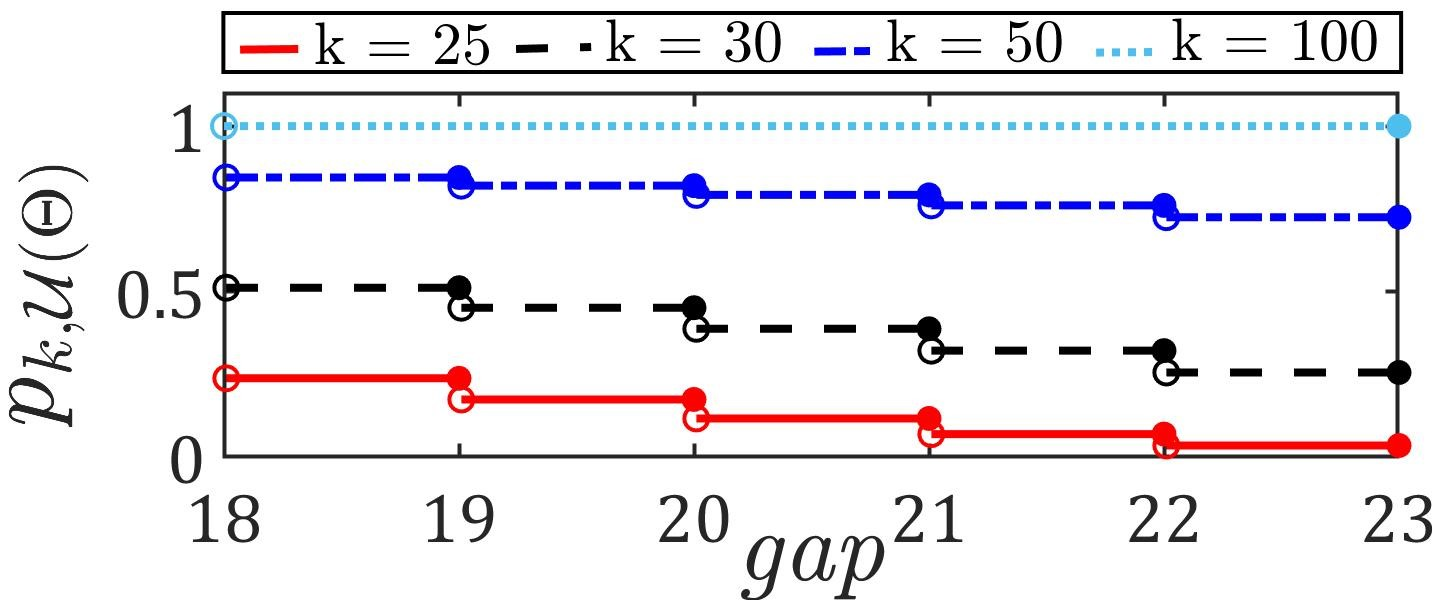
\includegraphics[width=\textwidth]{probs_time_horizon_Example2_New.jpg}
	\end{minipage}
	\caption{\textit{Left}: Model of  \SlplatoonTwo. \textit{Right}: Probability of hitting $\Unsafe$ vs. the initial $\mathit{gap}$ with different execution lengths $k$. Here, initial $s_1 \in  (20,23), s_2 \in  (0,2)$, $\mathsf{vb} = 1$, $\mathsf{vc} = 2$, $\mathsf{pfar} = 0.85$, $\mathsf{pnear} = 0.15$, $\mathsf{near} = 3$ and $\delta = 1$ }
	\label{fig:singlelane}
\end{figure}
%
 Let $s_{i}$ be the position of $i$\textsuperscript{th} car in the sequence. Initially, $s_i$ takes a value in an interval on the $x$-axis such that $s_{1} > s_{2} >\ldots > s_{m}$.
 % Sayan: Not sure that we need this.
%  and assume that cars can pass each other.
The pseudocode in Figure~\ref{fig:singlelane} specifies the probabilistic transition rule that updates the position of all the cars synchronously. Car $1$ always moves at a constant breaking speed of $\mathsf{vc}$.
%
The variable $\mathit{gap}_i$ is the distance of $i$ to the predecessor $i-1$, for each $i=2,...,m$.
If $\mathit{gap}_i$ is less than the constant threshold $\mathsf{near}$, then $i$ continues to cruise with probability $\mathsf{pnear}$ and it brakes with probability $1- \mathsf{pnear}.$
% pnear should be small,
% maybe use explicit numbers like 1/10
Similarly, if $\mathit{gap}_i$ greater than $\mathsf{near}$, then $i$ continues to cruise with probability $\mathsf{pfar}$ and brakes with probability $1- \mathsf{pfar}.$
% pfar should be large.

It is straightforward to connect the above  description to a formal definition of a \modelname. The state space  $\X=\mathbb{R}^m$. The set of initial states $\Theta$ is a hyperrectangle in  $\X$ (such that $s_1 > s_2 \ldots > s_m$). For any state, $x\in \X$ the probability transition function is given by the equations in lines~\ref{ln:lead_p}, \ref{ln:other_p1}, \ref{ln:other_p2}, \ref{ln:other_p3} and \ref{ln:other_p4}.
We define the set of unsafe states $\Unsafe =\{(s_{1},s_{2},...,s_{m})\in \X\ |\ \exists i\in\{2,...,m\},\ \mbox{ such that }\mathit{gap}_i  \leq \delta\}\subseteq \X$ for some constant collision threshold $\delta$.
% \sayan{Should we first consider an unsafe set where cars collide or get too close?}\textcolor{magenta}{I changed the definition of the unsafe set. Also in this case the leading car will always break instead of cruise. We also can change brake an cruise to cruise and speed up. }
% \geir{I dont see why we have the variable $t$ in the definition of $\mathcal{U}$; also do we want \emph{all} the cars to be less than
% $\delta$ from their predecessor for the unsafe set, or is it enough that one is too close?  Assuming both, it seems that the definition should simply be
% $\Unsafe =\{(s_{1},s_{2},...,s_{m})\in \X\ |\ \exists i\in\{2,...,m\},\ \mbox{ such that }\mathit{gap}_i  \leq \delta\}\subseteq \X$}

Given that cars start their motion at any initial state from $\Theta$, the goal is to find the maximum probability of hitting the unsafe set $\Unsafe$.
For $m=2$,
$\mathsf{vb} = 1$,
$\mathsf{vc} = 2$,
$\mathsf{pfar} = 0.85$
$\mathsf{pnear} = 0.15$,
$\mathsf{near} = 3$,
$\delta = 1$,
and initial $s_1 \in  (20,23), s_2 \in  (0,2)$,
Figure~\ref{fig:singlelane} shows estimates of probabilities of hitting the unsafe set from different initial separations between cars.
%
%p_{b,far} = 0.1$, $p_{b,near} = 0.9$, $p_{c,far} = 0.9$, $p_{c,near} = 0.1$ and $\delta = 5$.
As our intuition suggests, for large enough time horizons the probability of hitting the unsafe set approaches $1$ from all initial states, but, for smaller time horizons the maximum probability of unsafety arises when the initial gap is smaller.


\section{Statistical Model Checking with Optimistic Optimization}
%\input{multifid-back}
\subsection{Hierarchical Optimistic Optimization}
\label{sec:multi-fid-background}

{\em Multi-Fidelity Hierarchical Optimistic Optimization (MFHOO)}~\cite{sen2019noisy} is an black-box optimization algorithm from the  {\em multi-armed bandits} literature~\cite{munos:hal-2014,Bubeck:2011,Bubeck12}. The setup is the following: suppose we want to maximize the function $f:\X \rightarrow \mathbb{R}$, which is assumed to have a unique global maximum. Let $f^* = \underset{x\in\X}{\sup}$ $f(x)$. MFHOO allows the  choice of  evaluating  $f$ at different fidelities with different costs.
%
This flexibility matters for SMC  because it will be beneficial to evaluate the probability of unsafety $\phit{k}{x_0}{\Unsafe}$ for certain initial states more precisely, for example, with longer number of simulations, while for other initial states a less precise evaluation may be adequate.

Thus, MFHOO has access to a biased function $f_z(x)$ that depends on fidelity parameter $z \in [0,1]$.
%
Setting $z = 0$ gives the lowest fidelity (and lowest cost) and $z=1$ corresponds to full fidelity (and highest cost).
%
At full fidelity,  $f_1(x) = f(x)$, and the evaluation is unbiased. More generally, $|f_z(x)-f(x)|\leq\zeta(z)$ and evaluating $f_z(x)$ costs $\lambda(z)$, where the functions $\zeta, \lambda:[0,1]\rightarrow\mathbb{R}_{>0}$ are respectively,  non-increasing and non-decreasing, and called the {\em bias} and the {\em cost} functions~\cite{sen2019noisy}.

A bandit algorithm chooses a sequence of sample points (arms) $x_1, x_2, \ldots \in \X$, evaluates them at fidelities $z_1, z_2, \ldots$, and receives the corresponding sequence of noisy observations (rewards) $\observ_1, \observ_2, \ldots$.
%
%\marginnote{\scriptsize{\geir{We might want to comment here on this key property.}
%}}
%\textcolor{magenta}{
% \sayan{
% We assume that each $\observ_j$ is drawn from a distribution $M_{z_j,x_j}$ with  mean $f_{z_j}(x_j)$ and variance $\sigma^2$. That is, $f_{z_j}(x_j)= \int u dM_{z_j,x_j}(u)$.}
%\textcolor{magenta}{
We assume that each $\observ_j$ is drawn from a unknown distribution $M_{z_j,x_j}$ satisfying $f_{z_j}(x_j)= \int u dM_{z_j,x_j}(u)$. Further the distribution has a sub-Gaussian component, with variance $\sigma^2$, which captures uncertainty in the observations.
%}
%
%\marginnote{\scriptsize{\sayan{Trigger? Where do we need this $\epsilon,\sigma$? Isnt this a distribution on R+?}}}
%
The algorithm {\em actively chooses\/}  $x_{j+1}$ based on past  choices $x_1, \ldots, x_j$ and observations $\observ_1, \ldots, \observ_j$. When the budget $\Lambda$ is exhausted, the algorithm decides the optimal point $\bar{x}_{n(\Lambda)} \in \X$ and the optimal value $f(\bar{x}_{n(\Lambda)})$ with the aim of minimizing  {\em  regret\/}, which is defined as
\[
R(\Lambda)=f^*-f(\bar{x}_{n(\Lambda)}).
\]
% Unlike the typical SMC setting where the sampling strategy is fixed, in the bandit setting, the algorithm {\em actively chooses\/}  $x_{j+1}$ based on past  choices $x_1, \ldots, x_j$ and observations $\observ_1, \ldots, \observ_j$.
%
% A very short description of the key idea of HOO
The MFHOO algorithm (Algorithm~\ref{Al:MFHOO}) for selecting $x_{j+1}$ estimates $f^*$ by building a binary tree in which  each height in the tree represents a partition of the state space $\X$. The algorithm maintains estimates of an upper-bound on $f$ for each partition subset, and uses the principle of optimism for choosing the next sample $x_{j+1}$. That is, it chooses the samples in those partitions where the estimated upper-bounds are the highest.

Each node in the constructed tree is labeled by a pair of integers $(h, i)$, where $h$ is the height of the node in the tree, and $i$ satisfying $0\leq i\leq 2^h$ is its position within height level $h$. The root is labeled $(0,1)$, and each
%
node  $(h,i)$ can have two children $(h+1, 2i-1)$ and $(h+1, 2i)$.
%
Node  $(h, i)$ is associated with subset a of $\X$, denoted by  $\partition{h}{i}$, where $\partition{h}{i}=\partition{h+1}{2i-1}\cup \partition{h+1}{2i}$, and for each $h$ these disjoint subsets satisfy $\cup_{i=1}^{2^h} \partition{h}{i} = \X$. Therefore, larger values of $h$ represent finer partitions of $\X$.
%, and deeper nodes represent smaller subsets Geir: seems like this clause was redundant
%
%\sayan{
%The abstract presentation of the algorithm does not specify how each $\partition{h}{i}$ is split between its children.
%}
%, except that the resulting partitioning scheme must satisfy the exponentially shrinking property of Assumption~\ref{Ass:HOO2}.}

For each node $(h,i)$ in the tree, the algorithm maintains the following information:
\begin{inparaenum}[(i)]
\item $\counter{h}{i}$: the number of times the node is visited;
\item $\hat{f}_{h,i}$: the empirical mean of observations  over points visited in $\partition{h}{i}$; \item   $U_{h,i}$: an initial estimate of the maximum of $f$ over $\partition{h}{i}$; and
\item $B_{h,i}$: a tighter and optimistic upper bound on the maximum of $f$ over $\partition{h}{i}.$
\end{inparaenum}
%

The algorithm proceeds as follows. The $\mathit{tree}$ starts out with a single node, the root $(0,1)$, initializes the $B$-values of its two children $B_ {1,1}$ and $B_{1,2}$ to $+\infty$, and initializes the cost $C$ to $0$. At a high-level, in each iteration of the \textbf{while} loop (line~\ref{ln:mf_outerwhile}), the algorithm adds a new node $(\mathit{hnew},\mathit{inew})$ in the $\mathit{tree}$ and updates all of the above quantities for several nodes in  $\mathit{tree}$. In more detail, first a $\mathit{path}$ from the root to a leaf is found by traversing the child with the higher $B$-value (with ties broken arbitrarily). Let the child with the higher $B$-value of the traversed leaf  be $(\mathit{hnew},\mathit{inew})$ (line~\ref{ln:mf_path}). An arbitrary point $x$ in the partition of this node $\partition{\mathit{hnew}}{\mathit{inew}}$ is chosen (line~\ref{ln:mf_choose}). Then, this point is evaluated at fidelity $z_{hnew}=\zeta^{-1}(\nu\rho^{hnew})$ and a reward $\observ$ is received (line~\ref{ln:mf_recieve}). Next, $\mathit{tree}$ is extended by inserting $(\mathit{hnew},\mathit{inew})$ in the $\mathit{tree}$ (line~\ref{ln:mf_insert}) and for all the nodes $(h,i)$ in $\mathit{path}$ including $(\mathit{hnew},\mathit{inew})$, the $\counter{h}{i}$ and the empirical mean $\hat{f}_{h,i}$ are updated (line~\ref{ln:mf_update-path}). Finally, in line~\ref{ln:mf_update-tree}, for all nodes $(h,i)$ in $\mathit{tree}$, $U_{h,i}$  and $B_{h,i}$ are updated using the smoothness parameters $\nu_{1}>0$ and $\rho\in(0,1)$ and the parameter $\sigma$. Once the sampling budget $\Lambda$ is exhausted, a leaf with maximum $B$-value is returned by the Algorithm~\ref{Al:MFHOO}~\cite{sen2019noisy}.

%\vspace{-0.5cm}
\begin{algorithm}[ht!]
\caption{Multi-Fidelity Hierarchical Optimistic Optimization~\cite{sen2019noisy}}
\label{Al:MFHOO}
\begin{algorithmic}[1]
\State \textbf{input}: Budget: $\Lambda$, parameter: $\sigma$, bias $\zeta(.)$, cost $\lambda(.)$, smoothness params $\nu>0$ and $\rho\in(0,1)$
%\State \textbf{Output}:
\State $\mathit{tree} =\{(0,1)\}$, $B_{1,1}=B_{1,2}=\infty$, $C=0$
	\While{$C\leq \Lambda$} $\label{ln:mf_outerwhile}$
        \State $(\mathit{path}, (\mathit{hnew},\mathit{inew})) \gets \mathit{Traverse}(\mathit{tree})$ $\label{ln:mf_path}$
        \State $\textbf{choose}$
        $x\in\partition{\mathit{hnew}}{\mathit{inew}}$ $\label{ln:mf_choose}$
        \State $\textbf{query}$ $x$ at fidelity $z_{hnew} = \zeta^{-1}(\nu\rho^{hnew})$ and get observation $\observ$ $\label{ln:mf_recieve}$
        \State $C \leftarrow C + \lambda(z_{hnew})$ $\label{ln:mf_cost}$
    	\State $\mathit{tree.Insert}((\mathit{hnew},\mathit{inew}))$ $\label{ln:mf_insert}$
    	\ForAll{$(h,i)\in \mathit{path}$} $\label{ln:mf_update-path}$
        	\State $\counter{h}{i} \leftarrow \counter{h}{i} + 1$
            \State $\hat{f}_{h,i} \leftarrow (1- 1/\counter{h}{i})\hat{f}_{h,i} + \observ/\counter{h}{i}$
    	\EndFor
    	\State  $B_{\mathit{hnew}+1,2\mathit{inew}-1} \leftarrow +\infty$, $B_{\mathit{hnew}+1,2\mathit{inew}} \leftarrow +\infty$
    	\ForAll{$(h,i)\in \mathit{tree}$}  from  leaves up to  root:  $\label{ln:mf_update-tree}$
        	\State $U_{h,i} \leftarrow \hat{f}_{h,i} +\mathit{sqrt}(2\sigma^2\ln n/\counter{h}{i})+\nu\rho^h + \zeta(z_{h})$
            \State $B_{h,i} \leftarrow \min\{U_{h,i}, \max\{B_{h+1,2i+1}, B_{h+1,2i}\}\}$
    	\EndFor
	\EndWhile\\

	\Return $\underset{(h,i)\in \mathit{tree}}{\rm argmax}\ B_{h,i}$
	\end{algorithmic}
\end{algorithm}

\label{sec:smc-mfhoo}
%\sayan{Here let us just say that we are using MFHOO with. In the experiments section, we can talk about the modified version that is POO and MFPOO.}
We aim to solve the statistical model checking problem of  maximizing $\phit{k}{\Unsafe}{x}$ of Equation~(\ref{eq:SMCproblem}) for a given \modelname $\M$ and a time horizon $k$,  using  MFHOO.
%\sayan{changing $k_{max}$ to  $k$ here.}
%
In order to apply the MFHOO algorithm, one has to make several critical choices regarding the objective function, the budget, the cost, the parameters for fidelity and smoothness, and the multi-fidelity bias function. In this section we discuss the rationale behind our choices.
%\sayan{Let us then enumerate all the choices in this section.}

\subsection{Objective function, budget, cost, and fidelity}
\label{sec:objAndfid}

\paragraph{Fidelity parameter $z$.}
Consider a \modelname $\mathcal{M} = (\X, \Theta, P)$ with the unsafe set $\Unsafe \subseteq \X$. We have to maximize  $\phit{k_{\mathit{max}}}{\Unsafe}{x}$ over all initial states $x \in \Theta$, and for a long time horizon $k_{\mathit{max}}$.
%
Given $x\in \Theta$, the fidelity of evaluating $\phit{k_{\mathit{max}}}{\Unsafe}{x}$  will depend on the actual length of the simulations drawn for creating the observation $y$ for the state $x$.
%
Suppose we fix $k_{\mathit{min}}$ as the shortest  simulation to be used. We define the  fidelity of an observation (or evaluation) with simulations of length $k \in [k_{\mathit{min}}, k_{\mathit{max}} ]$ as $z=(k-k_{min})/(k_{min}-k_{max})$.
%
%Let $k$ be the variable defining the time horizon such that $k\in[k_{min}, k_{max}]$ for some $k_{min}<k_{max}$. We define the fidelity variable $z=(k-k_{min})/(k_{max}-k_{min})$.
% In case of HOO, the length of simulations will always be $k=k_{\mathit{max}}$ which corresponds to full fidelity $z = 1$.

\paragraph{Objective function $f$ and observations.}
A natural choice for the objective function  would be to define $f_{z=1}(x) := \phit{k_{max}}{\Unsafe}{x}$, for any initial state $x \in \Theta$.
%Here $f(x)=f_{1}(x) = \phit{k_{max}}{\Unsafe}{x}$.
Computing this  probability, however, is infeasible when the probability transition function $P_\M$ is unknown. Even if $P_\M$ is known, calculating $\phit{k}{\Unsafe}{x}$ involves summing over  many executions (as in~(\ref{eq:sumexecs})).
%
Instead, we take advantage of the fact that MFHOO can work with noisy observations. For any initial  $x \in \Theta$, and execution $\alpha \in \execs{x}(k)$ we define the observation:
\begin{align}
\Observ = 1 \ \mbox{if} \ \alpha \in \execs{x}(k,\Unsafe), \ \mathit{and} \ = 0 \ \mathit{otherwise}.
%\left\{
%	\begin{array}{ll}
%		1 & \mbox{if} \ \alpha \ \mbox{hits} \ \Unsafe, \\
%		0 & \mbox{otherwise}
%	\end{array}\right.
\end{align}
%
% \sayan{Please check this para.}
Recall that for a fixed initial states $x$, $\M$ is a Markov chain and defines a probability distribution over the set of executions $\execs{x}(k)$ as given by Equation~(\ref{eq:sumexecs}).
Thus, given an initial state $x$,
$\Observ=1$ with probability $\phit{k}{\Unsafe}{x}$, and $\Observ=0$ with probability $1-\phit{k}{\Unsafe}{x}$.
%
% \marginnote{\scriptsize{\sayan{What does ``at fidelity $z$'' mean here? Fidelity $z$ defines $k$, aren't they equal?}}}
%
That is, $\Observ$ is a Bernoulli random variable with mean $\phit{k}{\Unsafe}{x}$ at fidelity $z$.
In  MFHOO, once an initial state $x \in \partition{\mathit{hnew}}{\mathit{inew}}$ is chosen (line~\ref{ln:mf_choose}), we simulate $\M$ upto $k$ steps several times  starting from $x$  and calculate the empirical mean of $Y$, which serves as the noisy observation $y$ at fidelity $z$.


%  Using the MFHOO, this choice of reward leads estimating the maximum $\phit{k}{\Unsafe}{x}$ over all $x \in \Theta$. It is assumed if $\M$ hits the unsafe set it will stay there after.

% \sayan{Why is that important?} \textcolor{magenta}{It makes things easier: 1. It may be the case that some trajectories do hit the unsafe set before the time horizon k, then if we do not model the unsafe set as absorbing states then that trajectory can go out of the unsafe set but it doesn't change the fact that the trajectory has hit the unsafe set. I mean for us the reward is 1 either we consider this or not. It is just easier to model this way. 2. May be less important but computationally it can save time for large time horizons, when a trajectory hits the unsafe set we break the for loop. 3. It makes the analysis of multi fidelity bias function much easier.}
% \sayan{OK, let us move this ``absorbing'' $\Unsafe$ assumption to where it is really used}

% \textcolor{magenta}{I guess we need to define $z$ before cost function and multi-fidelity bias function}
% \sayan{Sure.}

% \paragraph{Cost $\lambda(\cdot)$, fidelity z, and budget $\Lambda$.}
% \sayan{Please check all of this.} For HOO, we measure cost  in terms of the number of individual states $x \in \Theta$ that are evaluated by the algorithm. The budget $N$ is set in terms of the number of states evaluated for regret bounds.

% \sayan{For MFHOO define fidelity, cost, and budget.}

%\input{experiments}
\section{\toolname{} tool and experimental evaluation}
\label{sec:experiments}
We have implemented a prototype tool called
\toolname\ which uses MFHOO for solving the SMC problem of~(\ref{eq:SMCproblem}). We  compare the performance of \toolname\ with that of  Prism~\cite{HKNP06}, Storm~\cite{dehnert2017storm}, and PlasmaLab~\cite{legay2016plasma} on several benchmarks we have created.

\subsection{Benchmark models}
\label{sec:allbenchmarks}
% \subsubsection*{Single-lane platoon with three modes: \SlplatoonThree}
We have created several \modelname models for evaluation of probabilistic and statistical model checking tools. The benchmarks are variants of \SlplatoonTwo. The executable models are available from~\cite{SMCOO-online:2020}.
% Dawei: Please create the bibentry for online artifacts.

\SlplatoonThree\ models a platoon of $m$ cars where in every time step, each car can choose to move with one of {\em three\/} speeds: $\mathsf{vbrake}$, $\mathsf{vcruise}$, and $\mathsf{vspeedup}$.
The first vehicle always moves at some constant speed. For all the others, these three actions are chosen probabilistically, according to probability distributions that depend on their distance to the preceding vehicle.
%
For example, if the distance $s_{i-1} - s_i$ is less than a threshold constant $\mathsf{th\_close}$ then the speed is chosen according to a probability distribution $\mathsf{pclose}$.

The state variables of the model are defined as follows: for the $i^{th}$ car, we denote $s_i \in \mathbb{R}$ as the position along the lane. With out loss of generality, we assume $s_1> s_2 > \ldots > s_m$. We also define an auxiliary variable $\mathit{gap}_i$ for all $i>1$ as the distance to the preceding car, i.e. $\mathit{gap}_i = s_{i-1} - s_i$. The set of initial states and the unsafe set have the same definition as in \SlplatoonTwo.

The constants in the model are defined as follows: $\mathsf{th\_far}$ and $\mathsf{th\_close}$ are some distance thresholds; $\mathsf{vbrake}$, $\mathsf{vcruise}$ and $\mathsf{vspeedup}$ are some velocities; $\mathsf{pclose}$, $\mathsf{pfine}$ and $\mathsf{pfar}$ are probability distributions for different modes. For example, $\mathsf{pclose}$ is the probability distribution over three actions, ``brake", ``cruise" and ``speed up", and we denote $\Pr(v=\mathsf{vbrake}) = \mathsf{pclose}[brake]$ as the probability of choosing action ``brake" when this probability distribution is used.

With these variables, the behavior of each car at every time step is described in Fig.~\ref{fig:Slplatoon3}.
%
\begin{figure}
	\centering
	\hrule
	\two{.3}{.70}
	{\lstinputlisting[language=pseudocode,lastline=10]{Slplatoon3.hioa.tex}}
	{\lstinputlisting[language=pseudocode,firstline=11, firstnumber=5]{Slplatoon3.hioa.tex}}
	\hrule
	\caption{Model of a platoon of cars on a single lane trying not to collide}
	\label{fig:Slplatoon3}
\end{figure}

% \subsubsection*{Multi-lane platoon: \Mlplatoon}
\Mlplatoon\ models a platoon of $m$ cars on $\ell$ lanes where in every time step, each car can choose to move with one of {\em five\/} actions: moving forward with speed $\mathsf{vbrake}$, $\mathsf{vcruise}$ or $\mathsf{vspeedup}$, or chaging to the left or right lane. These actions are chosen probabilistically, according to probability distributions that depend on their distances to the vehicles on its current lane, left lane or the right lane.

The state variables of the model are defined as follows: for the $i^{th}$ car, we denote $s_i \in \mathbb{R}$ as the position along the lane and $y_i \in \{1, \ldots, \ell\}$ as the ID of the current lane. Then, we define some auxiliary variables that can be derived from the state variables. We denote $\mathit{d\_ahead}[i]$ as the distance to the preceding car on the same lane. If the $i^{th}$ car is the leading car on its current lane, then $\mathit{d\_ahead}[i] = \infty$. Then, we denote $\mathit{d\_left}[i]$ as the minimal $s$-distance (i.e. only considering the difference of the $s$ variables) to the cars on the left lane. If there is no car on the left lane, then $\mathit{d\_left}[i] = \infty$. If the $i^{th}$ car is on the left-most lane, i.e. $y_i = 1$, then $\mathit{d\_left}[i] = -\infty$. Similarly, we define $\mathit{d\_right}[i]$.

The definition of the initial state space of this model is a little bit different due to the $y$ variables. When choosing the initial state, all the $y$ variables are set to 1, i.e. all cars start from the left-most lane. Then, $(s_1, \ldots, s_m)$ is picked from a rectangle in $\mathbb{R}^n$ just as what we have done in \SlplatoonTwo\ and \SlplatoonThree. Finally, we define the unsafe set $\Unsafe = \{(s_1, \ldots, s_m)\ |\ \exists i \in \{1, \ldots, m\}, \mathit{d\_ahead}[i] < \mathsf{unsafe\_rule}\}$.

The constants in the model are defined as follows: $\mathsf{th\_far}$, $\mathsf{th\_close}$ and $\mathsf{th\_clear}$ are some thresholds; $\mathsf{pturn}$ is the probability of chaning to the target lane if allowed to do that; $\mathsf{vbrake}$, $\mathsf{vcruise}$, $\mathsf{vspeedup}$, $\mathsf{pclose}$, $\mathsf{pfine}$ and $\mathsf{pfar}$ are defined with the same meaning as in \SlplatoonThree.

With these variables, the behavior of each car at every time step is described in Fig.~\ref{fig:Mlplatoon}.
%
\begin{figure}
	\centering
	\hrule
	\two{.3}{.70}
	{\lstinputlisting[language=pseudocode,lastline=11]{Mlplatoon.hioa.tex}}
	{\lstinputlisting[language=pseudocode,firstline=12, firstnumber=5]{Mlplatoon.hioa.tex}}
	\hrule
	\caption{Model of a platoon of cars on multiple lanes trying not to collide}
	\label{fig:Mlplatoon}
\end{figure}

\subsection{\toolname{} implementation and metrics}
\label{sec:eval-mfhoo}

Our implementation of the \toolname{} tool uses the MFHOO implementation presented in~\cite{sen2019noisy} to solve the model checking problem of Equation~(\ref{eq:SMCproblem}). It works in two stages: First, it uses MFHOO to find the best partition $\partition{h}{i}$ and a putative ``best" (most unsafe) initial point $x \in \partition{h}{i}$ with the maximum estimate for the probability of hitting the unsafe set $\Unsafe$. In the second stage, \toolname\ uses additional simulations to do a Monte Carlo estimation of the probability $\phit{k}{\Unsafe}{x}$. In the experiments reported below, a constant number of $26$K simulations are used in all experiments in the second stage.
%
% \marginpar{\scriptsize{\sayan{20K seems large. How sensitive are our results (quality, running time) to this number? How does this number compare with the number of sims in stage 1?}}}
%


To achieve the theoretically optimal performance, MFHOO  requires the smoothness parameters $\rho$ and $\nu$ which are unknown for our benchmarks. To circumvent this \toolname\ chooses  several parameter configurations ($3$ sets in our experiments), runs an instance of MFHOO for each, and  returns the result with the highest hitting probability. For each instance of MFHOO, we set a time budget which is the maximum time allowed to be consumed by the simulator.
% In our evaluation, we fix the number of instances of HOO to 3. Then, we set a time budget for the simulator, which is the total time consumed by the simulator.
% \marginpar{\scriptsize{\sayan{Check this para. Remind the reader how the regret is calculated. {\bf solution: A: added.}}}}


\paragraph{Metrics.}
We report the regret of \toolname. In order to calculate the regret, first we have to calculate the actual maximum hitting probability for each benchmark. This is computed using Prism~\cite{HKNP06} which uses numerical and symbolic analysis. The regret is the difference between the exact probability and the estimated probability. Then, we report the running time and memory usage. The memory usage is measured by calculating the total size of the Python object which contains the constructed tree and all other data of MFHOO. We also report the number of {\em queries\/} for each method, which is total number of simulations used in both stage 1 and 2.
%
All the experiments are conducted on a Linux workstation with two Xeon Silver 4110 CPUs and 32 GB RAM.

Table~\ref{tab:results} shows the running time, the memory usage, the number of queries, and the resulting actual regret for \toolname{} using MFHOO as well as \toolname(1) using HOO.
%
% \marginpar{\scriptsize{\sayan{queries not defined. Is this the number of simulations? In stage 1 or 2? both combined? {\bf solution: added. In Metrics.}}}}
%
On every benchmark, \toolname{} gives low regrets.
% \marginpar{\scriptsize{\sayan{For this to make sense, we should first say how regret was calculated...explicitly or using Prism. And relate the regret to the actual probability of hitting unsafe sets. {\bf solution: A: added. in metrics.}}}}
%
With the same simulation budget, \toolname{} devotes longer simulations in the interesting parts $\Theta$, as a consequence, it is usually faster than \toolname(1) as shown in Figure~\ref{fig:rescaling_comparison}.
% , which clearly verifies the efficiency of this multi-fidelity method.
%
% \marginpar{\scriptsize{\sayan{We need to talk about budget first. I'll have to revisit this last  para again. {\bf } }}}
%

% \sayan{MFHOO performance on 1 or 2 benchmarks,
% running time, budget, theoretical regret.}

% \sayan{Mention the type of computer used to perform all the experiments in the paper.}

\begin{table}[ht]
\scriptsize
\begin{center}
\begin{tabular}{|c|c|c|c|c|c|}
\hline
Model & Method & Time(s) & Memory(MB) & \#queries & Regret\\
\hline
\multirow{3}{*}{
	\begin{tabular}{c}
			\SlplatoonTwo \\
			$m=2$ \\
			$\phit{k_{\mathit{max}}}{\Unsafe}{x^*} = 0.8800$
	\end{tabular}
	}
 & Storm     & 68.88 & 1019 & NA & 0\\
                          & PlasmaLab & 37.73 & NA   & 749711  & 0.0017 $\pm$ 0.0020 \\
                          & \toolname(1) & 59.37 & 9.13 & 31381  & 0.0011 $\pm$ 0.0025\\
                          & \toolname    & 24.03 & 6.23 & \textbf{29415}   & \textbf{0.0002 $\pm$ 0.0020}\\
\hline
\multirow{3}{*}{
	\begin{tabular}{c}
			\SlplatoonThree \\
			$m=2$ \\
			$\phit{k_{\mathit{max}}}{\Unsafe}{x^*} = 0.8727$
	\end{tabular}
	}
 & Storm     & 89.10 & 1974 & NA & 0\\
                          & PlasmaLab & 22.61 & NA   & 749711 & 0.0022 $\pm$ 0.0021\\
                          & \toolname(1)       & 44.52 & 7.30 & 30315   & 0.0038 $\pm$ 0.0113\\
                          & \toolname     & 26.46 & 4.53 & \textbf{28520}   & \textbf{0.0010 $\pm$ 0.0018}\\
% \hline
% \multirow{3}{*}{
% 	\begin{tabular}{c}
% 			\SlplatoonThree \\
% 			$m=3$ \\
% 			$\phit{k_{\mathit{max}}}{\Unsafe}{x^*} = 0.8234$
% 	\end{tabular}
% 	}
%  & Storm     & NA & OOM & NA & NA\\
%                           & PlasmaLab & 23.78 & NA   & 749711 & 0.0021 $\pm$ 0.0022\\
%                           & \toolname(1) & 66.52 & 9.34 & 31487 & 0.0287 $\pm$ 0.0188\\
%                           & \toolname     & 56.25 & 8.72 & 30873 & 0.0126 $\pm$ 0.0203\\
\hline
\multirow{3}{*}{
	\begin{tabular}{c}
		\Mlplatoon\\
		$m=2,\ \ell=2$\\
		$\phit{k_{\mathit{max}}}{\Unsafe}{x^*} = 0.5918$
	\end{tabular}
	}
& Storm     & NA & OOM & NA & NA \\
                          & PlasmaLab & 49.14 & NA   & 749711 & 0.0032 $\pm$ 0.0026\\
                          & \toolname(1)       & 110.64 & 9.37 & 31555   & 0.0016 $\pm$ 0.0025\\
                          & \toolname     & 76.35 & 5.27 & \textbf{28955}   & \textbf{0.0007 $\pm$ 0.0043}\\
\hline
\end{tabular}
\end{center}
\caption{\small Comparison of \toolname{}, Storm and PlasmaLab. \toolname(1) corresponds to using HOO (i.e. the full fidelity algorithm) in stage 1 of \toolname. For regret of \toolname{} and PlasmaLab, we run the experiments for 10 times and report the ``mean $\pm$ std". For all the experiments, $|\overline{\Uptheta}| = 4096$.}
\label{tab:results}
\end{table}

\subsection{Comparison with other model checkers}
\label{sec:eval-mfhoo}
We compare the performance of \toolname{} with other model checkers. Prism~\cite{HKNP06} and Storm~\cite{dehnert2017storm} are leading probabilistic model checkers for Markov chains and MDPs and compute exact probability of reaching the unsafe states. As Storm has the same functionality as Prism and we found it to be much more efficient than Prism in all our experiments, we only compare \toolname\ with Storm.
%
% \marginpar{\scriptsize{\sayan{I have included Prism in the above sentence. Please check. {\bf solution: checked} {\bf Do we have to add Prism results? It is easy, but the results seem boring.}}}}
%
PlasmaLab~\cite{legay2016plasma} is one of the few  {\em statistical} model checkers that can handle MDPs. For probability estimation problems, PlasmaLab uses smart sampling algorithm~\cite{d2015smart} to efficiently assign the simulation budgets to each scheduler and then estimates the probability for the putative ``best" scheduler.

% \paragraph{Discretizing the initial set $\Theta$.} The theory for HOO and MFHOO is based on a continuous state space $\X$ and in our benchmarks the state variables are continuous. However, most probabilistic and statistical model checking tools, including the ones mentioned above, are designed for discrete state space models. Therefore, a straight-forward comparison of the approaches on the same model is infeasible, and we have to use discretized (quantized) versions of the benchmarks.

% For every benchmark, we first set all the constants in the model as integers, which leads to $\phit{k_{\mathit{max}}}{\Unsafe}{x}$ functions similar to the one shown in Figure~\ref{fig:singlelane}.
% %
% \marginpar{\scriptsize{\sayan{What functions? {\bf solution: added.}}}}
% %
% For any state $x \in \X$, there exists an integer state $\overline{x}$ such that $\phit{k_{\mathit{max}}}{\Unsafe}{x} = \phit{k_{\mathit{max}}}{\Unsafe}{\overline{x}}$.
% %
% \marginpar{\scriptsize{\sayan{Are we saying that by scaling the constants we create an equivalent model in which all the reachable states are always integers provided the initial state is also an integer?}}}
% %
% Therefore, we can discretize the initial state space $\Theta$ by only considering the integer initial states, and the maximal probability doesn't change. Denoting $\overline{\Theta}$ as the discretized initial state space, then we can construct an equivalent model with $\overline{\Theta}$ in model checkers like Storm or PlasmaLab which can only handle discrete models.

% \paragraph{Scaling the discrete initial state space.}
% Storm and PlasmaLab works on the discretized models while our method searches the continuous space directly. Thus, it is not fair to compare our method with others directly. In our method, the algorithm keeps partitioning $\Theta$ hierarchically and stops at a depth $h$, which can be considered as searching over all the $2^h$ partitions at depth $h$. In order to make a fair comparison, we scale the discrete model and get an equivalent discrete model for which $|\overline{\Theta}| = 2^h$. To do that, we first sample $2^h$ points uniformly in the continuous initial state space. Then we find an integer scaling factor $c$ such that by multiplying $c$ all the $2^h$ points become integer points. Other constants in the model are also multiplied by $c$. Then, all the Because $c$ is an integer, the constants in the model Then we evaluate Storm and PlasmaLab on the new model.
%
% \marginpar{\scriptsize{\sayan{This has to be explained more clearly. There are two things going on here. The integer states, and then the scaling. Let us discuss on skype. Or you can try to explain with an example.}}}
%

% \sayan{Say what we found about prisim.}
% \sayan{Say how you constructed the Storm / Plasma lab models.}

\paragraph{Discretizing and scaling the benchmarks.} The theory for  MFHOO is based on a continuous state spaces, however, most model checking tools, including the ones mentioned above, are designed for discrete state space models and they do not support floats as state variables. Therefore, a direct comparison of the approaches on the same model is infeasible, and we created equivalent, discretized (quantized) versions of the benchmarks.

In \toolname{}, the algorithm keeps partitioning $\Theta$ hierarchically and stops at a depth $h$, which can be considered as searching over all the $2^h$ partitions at depth $h$. In order to make a fair comparison, we make sure that the discrete version of the benchmark has $2^h$ initial states, i.e. $|\overline{\Theta}| = 2^h$ where $\overline{\Theta}$ is the discretized initial state space.

Before stating the discretizing process, we give two key observations of the benchmarks. First, considering the nature of our benchmarks, it is obvious that if we scale the velocities, distance thresholds and initial distances by a constant factor, the probability of hitting unsafe set doesn't change. Second, taking \SlplatoonTwo\ as an example, we set all the constants (velocities and distance thresholds) in the model as integers, which leads to the function $\phit{k_{\mathit{max}}}{\Unsafe}{x}$ shown in Figure~\ref{fig:singlelane}. It's clear that for any state $x \in \X$, there exists an integer state $\overline{x}$ such that $\phit{k_{\mathit{max}}}{\Unsafe}{x} = \phit{k_{\mathit{max}}}{\Unsafe}{\overline{x}}$. If we make sure that for each integer interval in the original continuous space, the discretized space has an value in that interval, then the maximum probability doesn't change. With these observations, we discretize the benchmark as follows. First, we sample $2^h$ points uniformly in the continuous initial state space. Due to the second observation mentioned above, if $2^h$ is larger than the number of integer points in the original space, the maximum probability doesn't change. Then, we find an integer scaling factor $c$ such that by multiplying $c$ all the $2^h$ points become integer points. Other constants in the model are also multiplied by $c$. According to the first observation, scaling with a constant doesn't change the probability. Thus, we now have a model where all state variables are integers and it has the same maximum probability as the original model. Then we evaluate Storm and PlasmaLab on this new model.

All of the model checkers mentioned above support the Prism~\cite{HKNP06} language. Thus, we implement each benchmark in Prism language, and then we check the equivalence between the Prism implementation and the Python implementation by calculating and comparing the probability $\phit{k_{\mathit{max}}}{\Unsafe}{x}$ at all integer points $x$.

For Storm, we report the running time and the memory usage. These metrics are directly measured by the software itself. For PlasmaLab, we report the running time. We do not report the memory usage of PlasmaLab because it doesn't provide an interface for that and it is hard to track the actual memory used by the algorithm inside the JAVA virtual machine. We also report the regret for PlasmaLab. We use the term ``regret" here just for simplicity, which also refers to the difference between the estimated probability and the exact probability.

The results of \toolname{}, PlasmaLab and Storm are summarized in Table~\ref{tab:results}. We show in Figure~\ref{fig:rescaling_comparison} how the performance of different methods changes as the $|\overline{\Uptheta}|$ increases. As the size of the initial state space increases, the memory usage of Storm grows quickly, which limits its application on large models. In contrast, \toolname{}  and PlasmaLab scale well. The running time of PlasmaLab is determined by the parameters of the smart sampling~\cite{d2015smart} algorithm. We use the same parameters regardless of $|\overline{\Uptheta}|$, and thus the running time of PlasmaLab is almost constant.

% TODO: results of \SlplatoonTwo.

As shown in Table~\ref{tab:results}, Storm fails to check the \Mlplatoon\ model due to the memory limitation. Compared with PlasmaLab, \toolname{} requires more running time.
%\sayan{On the other hand, the number of simulations used by PlasmaLab and the regret is higher than that of \toolname{}, for comparable running times (as we saw in Table~\ref{tab:results}.)}
%
However, we note that PlasmaLab is a considerably more mature tool than  \toolname.  As shown in Table~\ref{tab:results}, compared to PlasmaLab, \toolname{} requires much fewer queries to reach comparable regrets, which attests to the sample efficiency of our proposed method.

\begin{figure}[htbp]
    \centering
    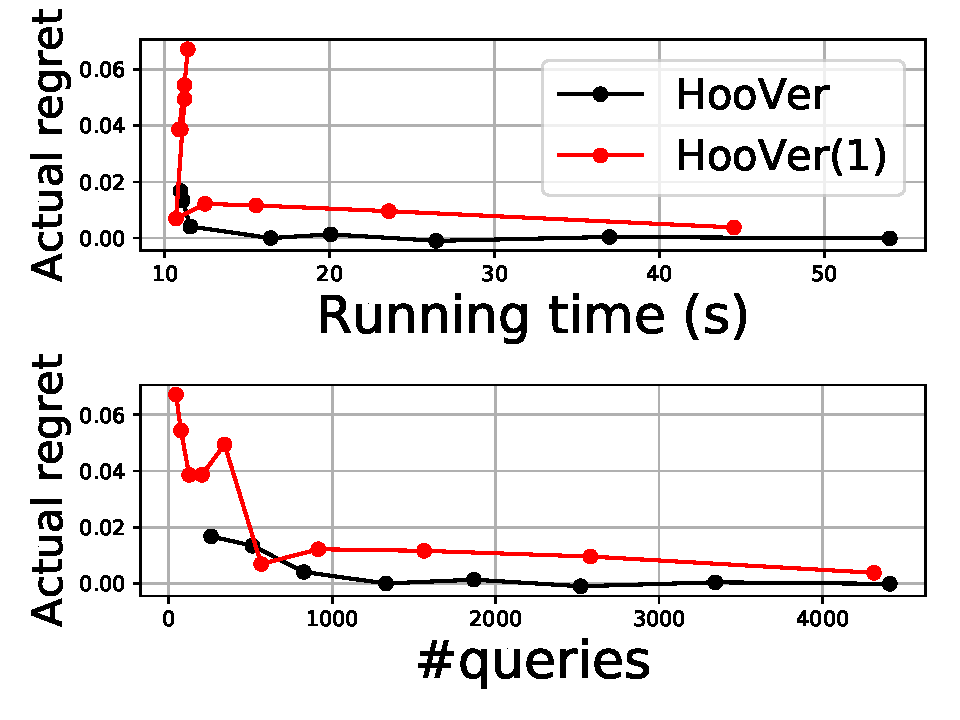
\includegraphics[width=0.32\textwidth]{comparison_HOO_MFHOO.pdf}
    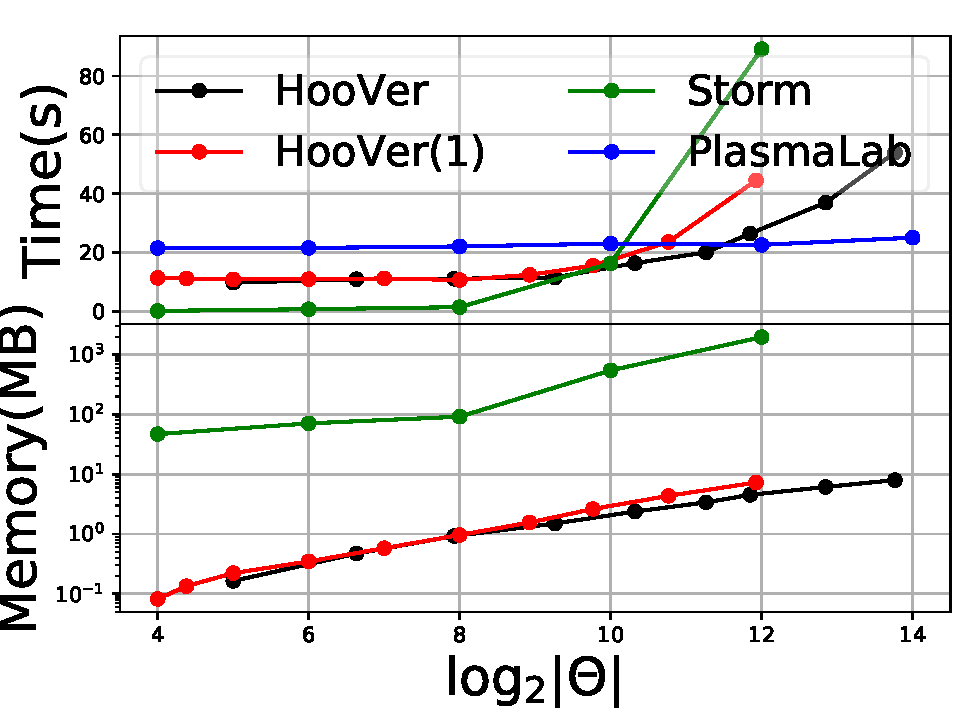
\includegraphics[width=0.32\textwidth]{rescaling_SLplatoon3_time_mem.pdf}
    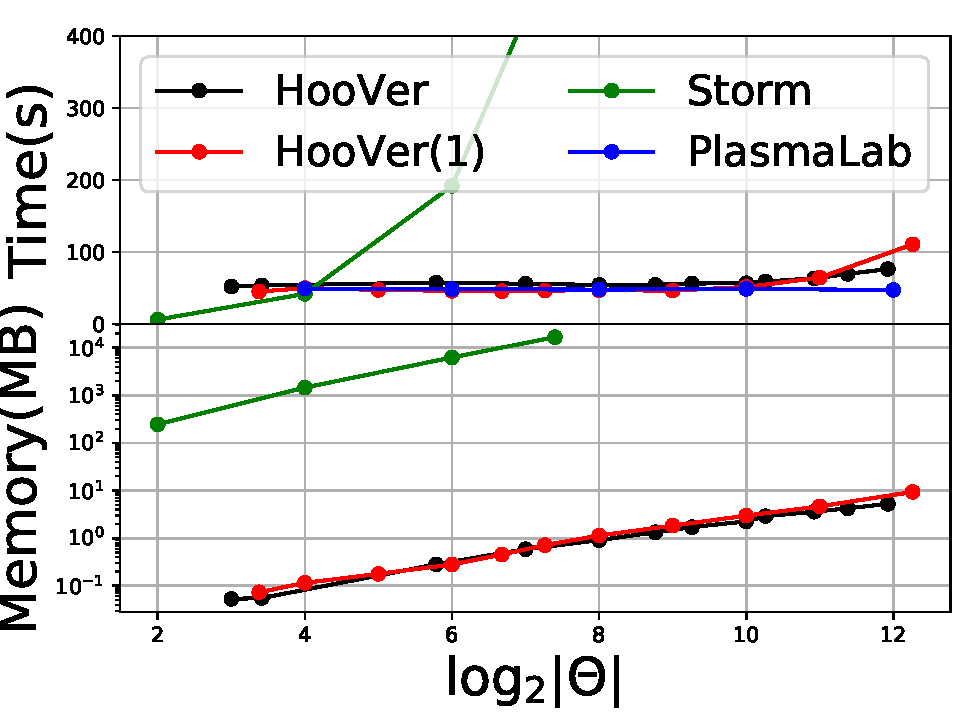
\includegraphics[width=0.32\textwidth]{rescaling_MLplatoon_time_mem.pdf}
    \caption{\small \textit{Left}: Comparison of \toolname{} and \toolname(1) on \SlplatoonThree. (Here, we only consider the number of queries in stage 1, because that for stage 2 is just a constant.) \textit{Middle}: Performance of different methods as the $|\overline{\Uptheta}|$ increases for \SlplatoonThree. \textit{Right}: Performance of different methods as the $|\overline{\Uptheta}|$ increases for \Mlplatoon.}
    \label{fig:rescaling_comparison}
\end{figure}



%\input{conclusions}
\section{Conclusions}
\label{sec:conc}
In this paper, we formulated the statistical model checking problem for a special type of MDP models as a multi-armed bandit problem and showed how a hierarchical optimistic optimization algorithm from~\cite{sen2019noisy} can be used to solve it. In the process, we modified the existing definition of near-optimality dimension to  accommodate  the  non-smoothness of the typical functions we have to optimize and recovered the regret bounds of the algorithm. We created several benchmarks, developed a SMC  tool \toolname{}, and experimentally established the sample efficiency and scalability of the method.

In order to enlarge the area of application of this method, it is necessary to study more general temporal properties for \modelname\ beyond bounded time safety. In this paper, we focused on a very special type of MDP models with nondeterminism only in the initial set. The results suggest that it will be  interesting to study black-box optimization algorithms for model checking more general MDP models.
%We did not try to optimize the performance of the tool, and we believe the tool could be more time efficient by reimplementing it carefully.

%https://www.overleaf.com/project/5cf027d15a966f3d04057872

%\newpage

%\input{appendix}

% The rest of the document

% Consider the discrete time Markov chain $\mathcal{M} = (\Omega, P, \Omega_0, \Omega_{US})$, with state space $\Omega$, unknown probability transition matrix $P$, set of initial states $\Omega_0 \subset \Omega$, and set of unsafe states $\Omega_{US} \subset \Omega$. The chain is a  sequence of states $(S_0, S_1, ... )$, where $S_0\in \Omega_0$. We define hitting probability, hitting time and expected hitting times for a state $x\in\Omega$ as:
% \begin{definition}\label{def:d1}
% The probability of hitting state $x\in\Omega$, given that chain starts at some state $y\in\Omega_0$, $P(y\rightarrow x)$ is defined as the probability that chain reaches state $x$ starting from state $y$. In other words, $P(y\rightarrow x) = P(S_t=x|S_0=y)$, where $t=min\{n\geq 0: S_n=x\}$.
% \end{definition}
% \begin{definition}\label{def:d2}
% Hitting time for $x\in \Omega$, $\tau_{x}$ is the first time that chain hits the state $x$. In other words, $\tau_{x} = min\{t\geq0:S_{t}=x\}$.
% \end{definition}
% \begin{definition}\label{def:d3}
% Expected value of $\tau_{x}$ given that chain starts from some state $y\in \Omega_0$ is $\mathbb{E}_{y}(\tau_{x}) = \mathbb{E}[\tau_{x}|S_{0}=y]$ for infinite time horizon.
% \end{definition}
% According to definitions \ref{def:d1}, \ref{def:d2} and \ref{def:d3}, for some state $y\in\Omega_0$, let $P(y\rightarrow \Omega_{US})$ and $\mathbb{E}_{y}(\tau_{us})$ be the probability of hitting unsafe set and expected hitting time of unsafe state, given that chain states at state $y$, respectively. Our objective is to determine the maximum probability of hitting the unsafe set within a predetermined time horizon, given that chain start from any state in initial set. In addition, determining the expected hitting time of the unsafe set within a predetermined time horizon is of our interest. In other word, we are interested in solving the following optimization problems within a specific time horizon:
% \begin{equation}
%   \underset{y\in\Omega_0}{\mathrm{max}}\ P(y\rightarrow \Omega_{US}),
% \end{equation}
% and
% \begin{equation}
%  \underset{y\in\Omega_0}{\mathrm{min}}\ \mathbb{E}_{y}(\tau_{us}).
% \end{equation}



\bibliographystyle{unsrt}
\bibliography{final}

\begin{appendices}

\section{Derivation of near-optimality dimension from Taylor expansion}
Near-optimality dimension is widely used in the proofs of the error bound of optimistic optimization methods \cite{munos2014bandits}. In this section, we give a simple method to calculate the  given the Taylor expansion at the optima.

\subsection{1-D case}
\begin{thm}
Considering a semi-metric $\ell(x, y) = ||x - y||_2^\beta$, a function $f: \mathbb{R} \mapsto \mathbb{R}$, the minimizer $x^* = \argmin\limits_{x \in \mathbb{R}} f(x)$, and the Taylor expansion of $f$ at $x^*$, $f(x) = f(x^*) + \sum\limits_{i = 1}^{\infty} c_i (x - x^*)^i$, if there exists an even number $\alpha \geq 2$ such that $c_\alpha \neq 0$ and $c_i = 0,\,\forall i<\alpha$, then the near-optimality of $f$ is $d = \frac{1}{\beta} - \frac{1}{\alpha}$.
\end{thm}

\begin{proof}
We have $f(x) - f(x^*) = c_\alpha (x-x^*)^\alpha + o((x-x^*)^\alpha)$. If $\epsilon$ is small enough, equation $f(x) - f(x^*) = \epsilon$ has two real roots $x^- \in (-\infty, x^*)$ and $x^+ \in (x^*, \infty)$, and $\mathcal{X}_\epsilon = [x^-, x^+]$. Because $c_\alpha (x^+-x^*)^\alpha + o((x^+-x^*)^\alpha) = \epsilon$, we have $\lim\limits_{\epsilon \downarrow 0} \left[ c_\alpha \frac{(x^+-x^*)^\alpha}{\epsilon} + \frac{o((x^+-x^*)^\alpha)}{\epsilon} \right] = 1$, and thus we must have $\lim\limits_{\epsilon \downarrow 0} \frac{(x^+-x^*)^\alpha}{\epsilon}$ exists and is not zero. Therefore, we have $\lim\limits_{\epsilon \downarrow 0} \frac{x^+ - x^*}{\epsilon^{1/\alpha}} = C_1 \neq 0$  Similarly, we have $\lim\limits_{\epsilon \downarrow 0} \frac{x^* - x^-}{\epsilon^{1/\alpha}} = C_2 \neq 0$. Then the near-optimality dimension is $d = \lim\limits_{\epsilon \downarrow 0} \frac{\ln \frac{(x^+ - x^*) + (x ^* - x^-)}{\epsilon^{1/\beta}}}{\ln \epsilon^{-1}} = \lim\limits_{\epsilon \downarrow 0} \frac{\ln \frac{(x^+ - x^*) + (x ^* - x^-)}{\epsilon^{1/\alpha}} + \ln \epsilon^{1/\alpha - 1/\beta}}{\ln \epsilon^{-1}} = \frac{1}{\beta} - \frac{1}{\alpha}.$
\end{proof}

\subsection{N-D case}
\begin{prop}
Considering a semi-metric $\ell(x, y) = ||x - y||_2^\beta$, a function $f: \mathbb{R}^D \mapsto \mathbb{R}$, the minimizer $x^* = \argmin\limits_{x \in \mathbb{R}^D} f(x)$, if the Taylor expansion of $f$ at $x^*$ is dominated by the $\alpha$-order term, then the near-optimality of $f$ is $d = D(\frac{1}{\beta} - \frac{1}{\alpha})$.
\end{prop}

\section{Usage of \toolname}
The code is available at \url{https://github.com/sundw2014/HooVer}.The MFTreeSearchCV code base was developed by Rajat Sen (\url{https://github.com/rajatsen91/MFTreeSearchCV}) which in-turn was built on the blackbox optimization code base of Kirthivasan Kandasamy (\url{https://github.com/kirthevasank}).

To run the existed benchmarks, run command like this:

\begin{verbatim}
python example.py --model [Slplatoon2/Slplatoon3/Mlplatoon]\
--budget [time budget for simulator] --numRuns [number of runs] [--useHOO]
\end{verbatim}

If ones want to add new benchmarks, they can create their own models following the interface used in models/Slplatoon2.py. For the Python implementation, the things that have to be defined include initial state space, step-forward simulation function, and the unsafe set.
\end{appendices}
\end{document}
